% ============================================================
%  PlanDiffusion 论文草稿
%  编译器：pdflatex / xelatex（推荐 xelatex，支持中文字体）
%  中文字体：宋体正文 / 黑体标题（需远端编译器安装 fandol 或系统中文字体）
% ============================================================

\documentclass[10pt,twocolumn,a4paper]{article}

% ── 中文支持（远端 Linux 编译器请确保安装 fandol 字体包）────────────────────
\usepackage[UTF8, fontset=fandol]{ctex}
% fandol 字体说明：
%   正文（宋体）→ FandolSong，等效宋体
%   粗体（黑体）→ FandolHei
%   斜体（楷体）→ FandolKai
% 若本地使用 xelatex + Windows 字体，可替换为：
%   \usepackage[UTF8]{ctex}
%   \setCJKmainfont{SimSun}[BoldFont=SimHei, ItalicFont=KaiTi   ]

% ── 页面设置（标准会议纸张：双栏，页边距约 1 inch）────────────────────────
\usepackage[
    a4paper,
    top=2.54cm, bottom=2.54cm,
    left=1.91cm, right=1.91cm,
    columnsep=0.64cm
]{geometry}

% ── 数学与符号 ──────────────────────────────────────────────────────────────
\usepackage{amsmath}
\usepackage{amssymb}
\usepackage{bm}          % 粗体数学符号

% ── 图表 ────────────────────────────────────────────────────────────────────
\usepackage{graphicx}
\usepackage{booktabs}    % 三线表
\usepackage{multirow}
\usepackage{array}
\usepackage[labelfont=bf, font=small, skip=4pt]{caption}
\usepackage{subcaption}

% ── 排版工具 ─────────────────────────────────────────────────────────────────
\usepackage{microtype}   % 微排版优化（西文）
\usepackage{xcolor}
\usepackage{verbatim}
\usepackage{enumitem}    % 列表间距控制
\setlist[itemize]{noitemsep, topsep=2pt}
\setlist[enumerate]{noitemsep, topsep=2pt}

% ── 算法 ────────────────────────────────────────────────────────────────────
\usepackage{algorithm}
\usepackage{algorithmic}

% ── 超链接（草稿用，投稿前检查是否需要去掉）─────────────────────────────────
\usepackage[colorlinks=true, linkcolor=blue, citecolor=blue, urlcolor=blue]{hyperref}

% ── 节标题格式：黑体，间距紧凑 ──────────────────────────────────────────────
\usepackage{titlesec}
\titleformat{\section}{\large\bfseries}{\thesection}{0.5em}{}
\titleformat{\subsection}{\normalsize\bfseries}{\thesubsection}{0.5em}{}
\titleformat{\subsubsection}{\normalsize\bfseries}{\thesubsubsection}{0.5em}{}
\titlespacing{\section}{0pt}{6pt}{3pt}
\titlespacing{\subsection}{0pt}{4pt}{2pt}
\titlespacing{\subsubsection}{0pt}{3pt}{1pt}

% ── 段落与行距 ───────────────────────────────────────────────────────────────
\usepackage{setspace}
\setstretch{1.05}        % 行距约 1.05 倍（会议标准为单倍，可调为 1.0）
\setlength{\parskip}{0pt}
\setlength{\parindent}{1em}

% ── 摘要样式（双栏摘要）────────────────────────────────────────────────────
\usepackage{abstract}
\renewcommand{\abstractnamefont}{\normalfont\bfseries}
\renewcommand{\abstracttextfont}{\normalfont\small}
\setlength{\absleftindent}{0pt}
\setlength{\absrightindent}{0pt}

% ── 参考文献间距 ────────────────────────────────────────────────────────────
\usepackage[numbers,sort&compress]{natbib}
\setlength{\bibsep}{2pt}

% ── 草稿辅助命令 ────────────────────────────────────────────────────────────
\newcommand{\todo}[1]{\textcolor{red}{\textbf{[TODO: #1]}}}

% ============================================================
%  标题 / 作者
% ============================================================
\title{
    \vspace{-1em}
    {\large \textbf{PlanDiffusion：基于自回归图结构生成与}}\\[2pt]
    {\large \textbf{坐标扩散的文本驱动住宅平面图生成}}
    \vspace{-0.5em}
}

\author{
    \todo{作者信息}
}

\date{}

% ============================================================
\begin{document}

\maketitle
\thispagestyle{empty}

% ── 摘要 ────────────────────────────────────────────────────────────────────
\begin{abstract}
\todo{等实验结果后填写。三句话结构：问题与现有局限 → 本文方法 → 实验结果。}
\end{abstract}

% ── 正文各节 ────────────────────────────────────────────────────────────────
\section{引言}
\label{sec:introduction}

住宅平面图的自动化生成是计算机辅助建筑设计的核心问题之一。
理想的系统应当允许设计师以自然语言表达设计意图
（如"客厅居中，两侧各有一间卧室，厨房通过走廊与卫生间相连"），
并自动生成与描述一致、拓扑合理的矢量平面图。

早期工作主要依赖图约束或气泡图（bubble diagram）作为生成条件~\cite{nauata2020housegan,shabani2023housediffusion}。
这类方法虽能输出几何上连贯的平面图，
但气泡图本身仍需由设计师手工绘制，并未从根本上解决"从语言到图纸"的端到端生成问题。
Architext~\cite{galanos2023architext} 率先将大语言模型引入平面图生成，
但其文本描述由规则模板自动生成，语言单一，与真实设计需求存在较大差距。
ChatHouseDiffusion~\cite{qin2025chathousediffusion} 进一步引入 prompt 引导并支持局部编辑，
但侧重于像素级图像生成，尚未面向矢量图结构的显式拓扑建模。

本文提出 \textbf{PlanDiffusion}，一种以\textbf{图结构为中间表示}的文本驱动平面图生成框架，
整体流程如图~\ref{fig:overview} 所示。
核心思路是将生成任务分解为三个串联阶段：
（1）\textbf{图拓扑生成}：以 LLaMA 自回归模型将文本描述转化为平面图的拓扑图结构，
包括节点数量与邻接关系；
（2）\textbf{节点坐标扩散}：以图结构和文本为双重条件，
通过去噪扩散概率模型（DDPM）生成每个顶点的二维坐标；
（3）\textbf{节点类型预测}：以生成坐标、图结构和文本为条件，
通过独立分类器预测每个节点的房间组合类型。
显式的图结构中间表示使拓扑约束在扩散过程中始终可控，
同时为坐标生成提供了强结构先验；
类型预测与坐标扩散完全解耦，在干净坐标上以纯监督方式训练。

为支撑上述框架的训练，我们在 Architext\_v1~\cite{galanos2023architext} 基础上构建了
\textbf{PlanText-150K}，一个包含 \textbf{149,950} 条样本的大规模平面图-文本数据集。
与原始数据集的模板式描述不同，
我们调用 MiMo-V2.5 视觉语言模型对每张平面图生成自然语言描述，
并经人工抽查校正，显著提升了文本标注的多样性与自然度。

本文的主要贡献如下：
\begin{itemize}
    \item 提出以图结构为中间表示的三阶段文本驱动平面图生成框架，
    在保证拓扑合法性的同时实现端到端的语言条件生成；
    \item 设计了"BFS 生成树 + 补边"的图序列化格式，
    使任意连通图均可被自回归语言模型高效建模；
    \item 构建了 PlanText-150K 数据集，
    通过 MiMo-V2.5 VLM 自动标注并经人工抽查校正提供高质量自然语言描述，
    是目前规模最大的带文本标注的住宅平面图数据集之一；
    \item 设计了三流注意力去噪网络（NodeDiffusionTransformer），
    并联邻接局部注意力（AdjAttn）、面结构注意力（RoomAttn）与全局注意力（GlobalAttn），
    分别捕捉节点的局部边约束、房间面约束与全局布局信息，
    在纯文本条件下高精度恢复节点坐标；
    并在此基础上扩展四流轮廓条件变体（PlanDiffusion-bnd），
    以外轮廓节点固定 + BndAttn 提供等价于 ChatHouseDiffusion 轮廓输入的几何约束，
    实现公平定量对比。
\end{itemize}

\begin{figure}[t]
    \centering
    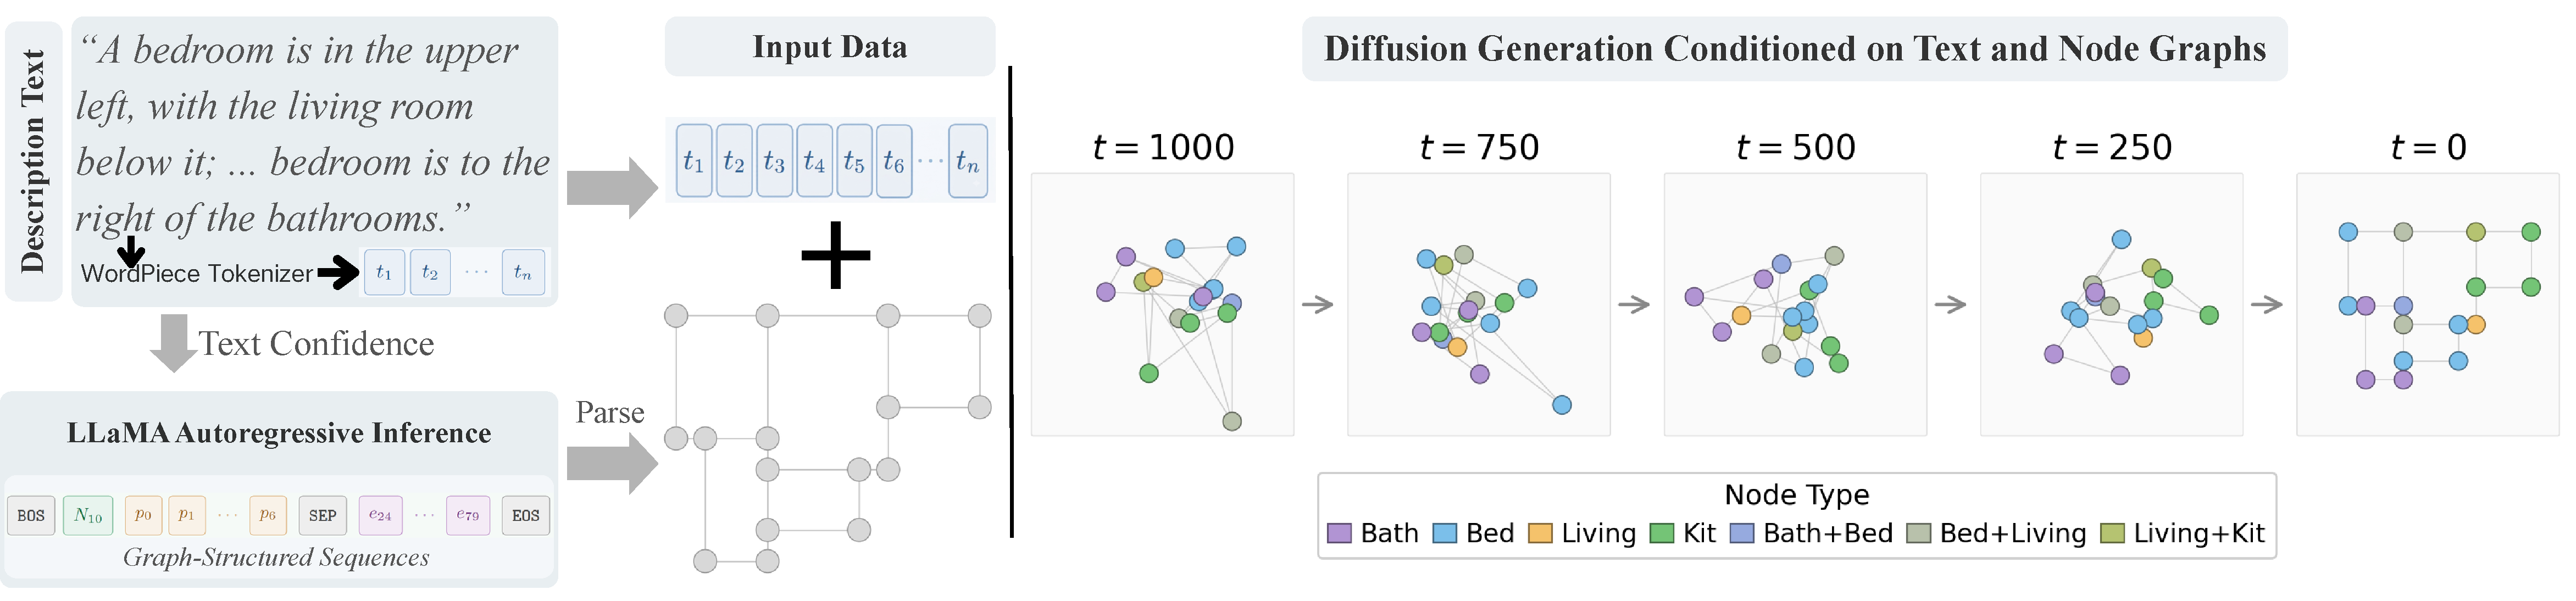
\includegraphics[width=\textwidth]{figures/total_process.pdf}
    \caption{
        PlanDiffusion 整体流程。
        左：图拓扑生成阶段以文本描述为条件，通过 LLaMA 自回归推理生成图结构序列，
        解析得到顶点图；
        右：完整三阶段生成过程——$\theta_2$ 以顶点图和文本为条件，
        通过 DDPM 逆扩散从高斯噪声（$t=1000$）逐步恢复节点坐标（$t=0$）；
        随后 $\theta_3$ 对节点进行类型预测，最终通过半边遍历与投票渲染输出彩色平面图。
    }
    \label{fig:overview}
\end{figure}

\section{相关工作}
\label{sec:related_work}

\subsection{平面图生成}
\label{subsec:floorplan_gen}

平面图生成方法大致可分为三类。

\textbf{图约束方法。}
House-GAN~\cite{nauata2020housegan} 将房间邻接图作为条件，
以关系生成对抗网络生成各房间的边界框，
开创了以图约束驱动布局生成的范式。
该类方法对拓扑结构有强控制能力，
但需要用户预先提供手绘气泡图，限制了易用性。

\textbf{扩散模型方法。}
HouseDiffusion~\cite{shabani2023housediffusion} 提出混合扩散模型，
在连续坐标与离散房间标签上联合去噪，
直接生成矢量多边形，取得了当时最优的几何质量。
其同样以气泡图为输入条件，不支持自然语言驱动。

\textbf{语言驱动方法。}
Architext~\cite{galanos2023architext} 在 250k 合成平面图上微调 GPT 系列模型，
实现了从自然语言描述到平面图的直接生成。
Tell2Design~\cite{leng2023tell2design} 构建了语言引导平面图数据集并探索了多种基线方法。
ChatHouseDiffusion~\cite{qin2025chathousediffusion} 将扩散模型与 prompt 引导相结合，
支持生成与编辑，但仍缺乏对拓扑结构的显式约束。

与上述工作不同，本文在文本和坐标之间引入显式图结构作为中间表示，
同时具备语言可控性和拓扑保证。

\subsection{自回归图结构生成}
\label{subsec:autoregressive_graph}

将图结构序列化后用自回归模型建模是图生成的经典思路。
You et al.~\cite{you2018graphrnn} 提出 GraphRNN，
以节点-边交替序列逐步生成图结构。
近年来，基于 Transformer 的方法进一步提升了序列建模能力。
DiGress~\cite{vignac2022digress} 将图生成建模为离散扩散过程，
在分子图和场景图上取得了优秀结果。
GRAN~\cite{liao2019gran} 通过自回归块生成稠密图，提升了效率。

本文的图序列化方案受"将图展平为序列"思路的启发~\cite{you2018graphrnn}，
采用"BFS 生成树 + 补边"格式，
使生成树部分（长度固定为 $N-1$）与补边部分（长度可变）结构清晰，
便于自回归模型学习。

\subsection{扩散模型在布局生成中的应用}
\label{subsec:diffusion_layout}

DDPM~\cite{ho2020ddpm} 提出去噪扩散概率模型后，
扩散过程被广泛应用于图像、点云、分子构象等结构化数据的生成。
在布局生成方向，LayoutDM、DiffLayout 等工作将扩散模型引入
UI 布局、文档排版等任务，取得了较好的多样性与质量均衡。
HouseDiffusion~\cite{shabani2023housediffusion} 将其引入矢量平面图，
验证了扩散模型在几何生成上的优越性。

本文的节点坐标扩散模块在 DDPM 框架下，
以图结构（邻接矩阵）和文本（WordPiece token）为双重条件，
通过双流注意力机制同时捕捉局部几何约束和全局语义信息，
与上述工作在条件化方式上存在本质区别。

\section{方法}
\label{sec:method}

\subsection{问题定义}
\label{subsec:problem}

给定自然语言描述 $\mathcal{T}$，目标是生成对应的住宅平面图。
我们将平面图表示为带属性的图 $\mathcal{G} = (\mathcal{V}, \mathcal{E})$，
其中 $\mathcal{V}$ 为节点集合（房间多边形的角点），
$\mathcal{E}$ 为边集合（相邻角点间的连接关系）。
每个节点 $v_i$ 附带二维坐标 $\mathbf{c}_i \in \mathbb{R}^2$ 和
组合类型标签 $y_i \in \{1, \ldots, 32\}$，
令 $\mathbf{X} = [\mathbf{c}_1, \ldots, \mathbf{c}_N]^\top \in \mathbb{R}^{N \times 2}$，
邻接矩阵 $\mathbf{A} \in \{0,1\}^{N \times N}$。

目标是学习联合分布 $p(\mathbf{A}, \mathbf{X}, \mathbf{y} \mid \mathcal{T})$，
我们将其分解为两个串联子问题：
\begin{equation}
    p(\mathbf{A},\mathbf{X},\mathbf{y} \mid \mathcal{T})
    = \underbrace{p_{\theta_1}(\mathbf{A} \mid \mathcal{T})}_{\text{Stage 1}}
    \cdot
    \underbrace{p_{\theta_2}(\mathbf{X}, \mathbf{y} \mid \mathbf{A}, \mathcal{T})}_{\text{Stage 2}}
    \label{eq:factorize}
\end{equation}
（1）\textbf{图拓扑生成}：自回归建模 $p_{\theta_1}(\mathbf{A} \mid \mathcal{T})$，
输出图的连接结构；
（2）\textbf{节点坐标与类型扩散}：以 $(\mathbf{A}, \mathcal{T})$ 为条件，
通过扩散模型建模 $p_{\theta_2}(\mathbf{X}, \mathbf{y} \mid \mathbf{A}, \mathcal{T})$。

% -----------------------------------------------------------------------------
\subsection{数据集}
\label{subsec:dataset}

\begin{figure}[htbp]
    \centering
    
\includegraphics[width=\linewidth]{figures/dataset_fig.pdf}
    \caption{
        数据集样例。每条样本包含住宅平面图渲染（左）、
        对应顶点图表示（中）及 VLM 自动生成的自然语言描述（右）。
        顶点颜色表示组合类型，边表示几何连接关系。
    }
    \label{fig:dataset}
\end{figure}

现有平面图数据集的文本标注普遍依赖规则模板，语言单一，且缺乏结构化的图表示。
Architext\_v1~\cite{galanos2023architext} 虽提供大规模合成平面图，
但其描述仅为简单模板句（如 ``a house with two bedrooms and one bathroom''），
不足以支撑文本条件生成的训练。
为此，我们在 Architext\_v1 基础上构建了新的训练数据集，
引入顶点图表示与 VLM 生成的自然语言描述，如图~\ref{fig:dataset} 所示。

\paragraph{顶点图表示}
我们将平面图表示为\textbf{顶点图}：
以房间多边形的全部角点为节点，以多边形边上相邻顶点的连接为边。
由于多个房间可能共享同一顶点（如卧室与走廊的公共墙角），
每个节点的类型定义为其所属全部房间类型的有序组合，
称为\textbf{组合类型（combo type）}。
与使用房间中心点的方案相比，
顶点图保留了平面图完整的几何拓扑信息，
并使图结构与几何形状之间保持一一对应。
全部训练样本中共出现 32 种组合类型，每种分配唯一整数 ID（1--32）。

\paragraph{自然语言标注}
我们将顶点图渲染为彩色平面图图像，
调用多个视觉语言模型（Qwen 系列、DeepSeek-V3、Kimi 等，共 40 余个）
对每张图生成自然语言描述，并按模型质量优先级选取最佳结果。
标注要求直接陈述各房间的位置关系与连通关系，
回避视觉指代词，使描述可独立于图像作为文本条件使用。

\paragraph{统计}
最终数据集包含 \textbf{149,609} 条样本，
每条样本含邻接矩阵（$40{\times}40$）、节点坐标（$40{\times}2$）、
组合类型 ID（$40$）及文本描述（WordPiece 编码，训练截断至 128 token）。
数据集关键统计如表~\ref{tab:dataset_stats} 所示。

\begin{table}[h]
\centering
\caption{数据集统计}
\label{tab:dataset_stats}
\small
\begin{tabular}{lrrr}
\toprule
统计项 & 最小 & 均值 & 最大 \\
\midrule
样本总数           & \multicolumn{3}{c}{149,609} \\
节点数             & 9    & 22.4 & 40  \\
边数               & 12   & 28.6 & 49  \\
文本长度（token）  & 33   & 81.8 & 145 \\
单类型节点占比     & \multicolumn{3}{c}{60.7\%} \\
多类型节点占比     & \multicolumn{3}{c}{39.3\%} \\
Combo 类型总数     & \multicolumn{3}{c}{32} \\
\bottomrule
\end{tabular}
\end{table}

% -----------------------------------------------------------------------------
\subsection{统一词表}
\label{subsec:vocab}

为使文本 token 与图结构 token 共存于同一序列空间，
我们采用 BERT-base-uncased 的前 10,000 个 WordPiece token 作为文本词表，
并在其后追加 84 个图结构专用 token，构成大小为 10,084 的统一词表，
具体如表~\ref{tab:vocab} 所示。
该词表同时被 Stage~1 和 Stage~2 共享。
相较于在领域数据上重新训练 BPE，直接复用 BERT WordPiece 词表使系统更易与
预训练语言模型对接，且对英文建筑描述具有良好的覆盖率。

\begin{table}[h]
\centering
\caption{统一词表布局}
\label{tab:vocab}
\small
\begin{tabular}{lll}
\toprule
ID 范围 & Token & 说明 \\
\midrule
0 -- 9999    & WordPiece token & 文本词表（BERT 前 10k）\\
10000        & \texttt{PAD}    & 填充 \\
10001        & \texttt{BOS\_G} & 图序列起始 \\
10002        & \texttt{EOS\_G} & 图序列终止 \\
10003        & \texttt{SEP}    & 生成树与补边分隔符 \\
10004--10043 & $N_k$           & 节点数量（$N=1{\sim}40$） \\
10044--10083 & 节点 token       & 节点编号（$0{\sim}39$） \\
\bottomrule
\end{tabular}
\end{table}

% -----------------------------------------------------------------------------
\subsection{阶段一：自回归图拓扑生成}
\label{subsec:llm_graph}

\subsubsection{图序列化格式}

给定含 $N$ 个节点的图，我们将其序列化为：

\begin{equation}
\small
\underbrace{t_1 \cdots t_L}_{\text{BPE 文本}}\;
\texttt{BOS\_G}\;
\underbrace{N_k}_{N \text{ 个节点}}\;
\underbrace{p_1 \cdots p_{N-1}}_{\text{生成树父节点}}\;
\texttt{SEP}\;
\underbrace{i_1\, j_1 \cdots}_{\text{补边}}\;
\texttt{EOS\_G}
\label{eq:seq}
\end{equation}

其中生成树通过 BFS 遍历构建，父节点序列 $p_i = \texttt{NODE} + \mathrm{parent}(i)$
记录每个节点在 BFS 树中的父节点；
补边为不属于生成树的额外边，每条边用两个 token 表示。
这一"生成树 + 补边"格式结构规整（父节点序列长度固定为 $N-1$），
且任意连通图均可唯一表示。
为增强多样性，对每张图从不同起始节点执行 BFS（增强 ${\times}4$）。

图~\ref{fig:seq_graph} 展示了自回归生成过程中图结构的逐步构建：
从部分父节点序列对应的局部生成树，到完整生成树，再逐步添加补边，
最终恢复完整图拓扑。

\begin{figure}[t]
    \centering
    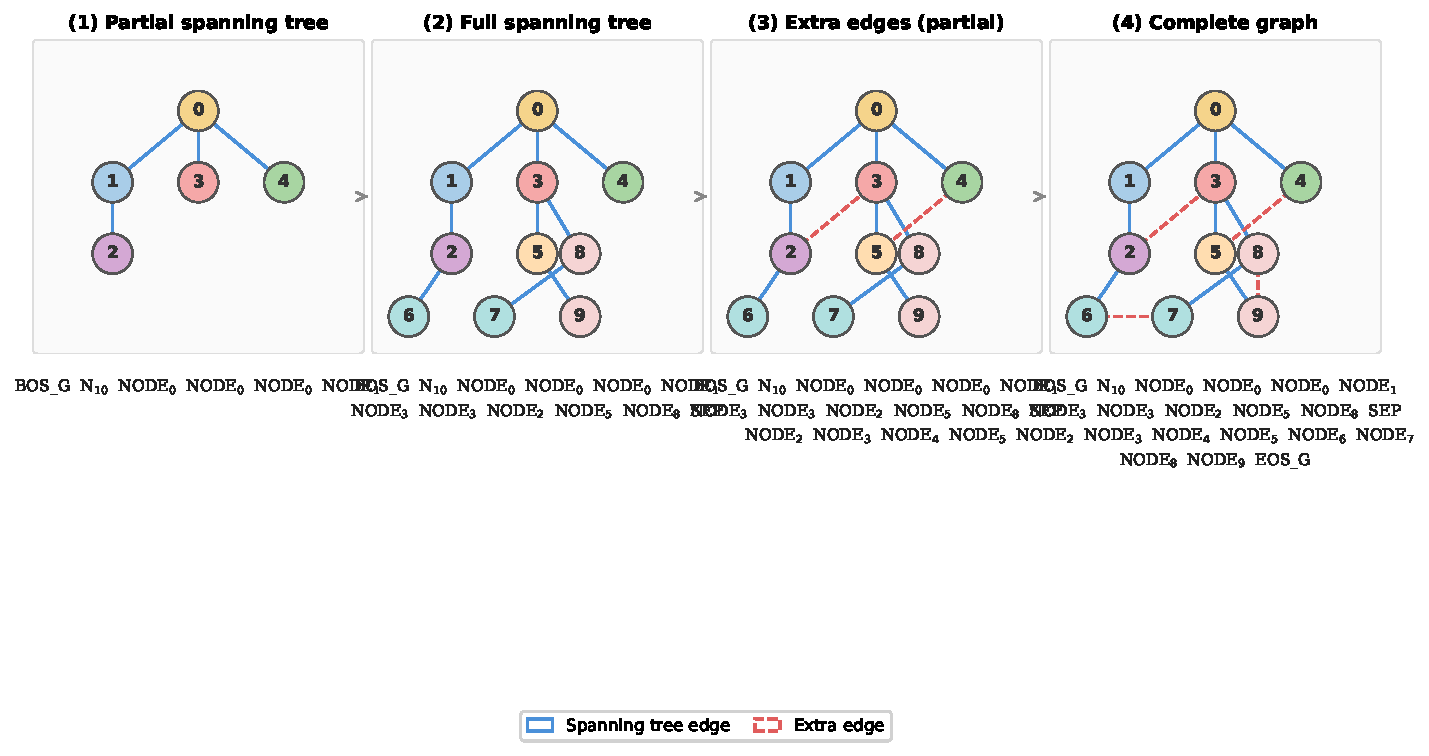
\includegraphics[width=\linewidth]{figures/seq_graph.pdf}
    \caption{
        图序列化的自回归生成过程（真实数据，$N=10$）。
        蓝色实线为 BFS 生成树边，红色虚线为补边。
        从左至右依次为：
        （1）生成部分父节点 token 后的局部生成树；
        （2）父节点序列生成完毕（\texttt{SEP} 前）的完整生成树；
        （3）生成前两条补边后的图；
        （4）所有补边生成完毕（\texttt{EOS\_G} 前）的完整图。
    }
    \label{fig:seq_graph}
\end{figure}

令 $\mathbf{s} = (s_1, \ldots, s_K)$ 为完整序列（含文本前缀），
模型建模：
\begin{equation}
    p_{\theta_1}(\mathbf{A} \mid \mathcal{T})
    = \prod_{k \in \mathcal{I}_g} p_{\theta_1}(s_k \mid s_{<k})
    \label{eq:ar}
\end{equation}
其中 $\mathcal{I}_g$ 为 $\texttt{BOS\_G}$ 之后的图 token 下标集合；
文本部分 label 置 $-100$，不计入 loss。

\subsubsection{模型结构}

本阶段采用 \texttt{LlamaForCausalLM}~\cite{touvron2023llama} 为自回归主干，
配置为：隐藏层维度 512，8 层，8 头，前馈维度 1536，
词表大小 10,084，约 20M 参数。

\subsubsection{两阶段训练策略}

直接在文本+图联合序列上训练易导致模型难以同时学习语言理解与图结构生成。
为此，我们采用两阶段训练：

\textbf{预训练（图结构预训练）}：
仅使用图序列部分（\texttt{BOS\_G} 之后），
令模型在不依赖文本条件的情况下先学习图结构语法，
训练 50 epoch。

\textbf{微调（文本条件微调）}：
以预训练权重初始化，输入完整文本+图联合序列，
loss 仅在图序列部分计算，训练 100 epoch。

两阶段均采用 AdamW（$\beta_1{=}0.9$，$\beta_2{=}0.95$，
lr $= 10^{-4}$，余弦退火至 $10^{-5}$），
grad clip $= 1.0$，FP16 混合精度。

% -----------------------------------------------------------------------------
\subsection{阶段二：节点坐标与类型联合扩散}
\label{subsec:node_diffusion}

\subsubsection{联合扩散对象}

坐标 $\mathbf{x}_0 \in \mathbb{R}^{2 \times N}$ 可直接在欧氏空间扩散。
类型标签 $y_i \in \{1,\ldots,32\}$ 为离散量，无法直接施加高斯噪声；
为此，我们将其映射到连续嵌入空间：
\begin{equation}
    \mathbf{e}_0^{(i)} = \mathrm{Emb}(y_i) \in \mathbb{R}^{d},
    \quad d = 384
    \label{eq:type_emb}
\end{equation}
并在嵌入空间对 $\mathbf{e}_0^{(i)}$ 施加高斯扩散。
这使坐标与类型可在统一的 Gaussian DDPM 框架下联合训练，
无需引入离散扩散机制。

\subsubsection{前向过程}

采用线性 beta 调度（$\beta_t \in [10^{-4},\, 0.02]$，$T=1000$），
令 $\alpha_t = 1 - \beta_t$，$\bar{\alpha}_t = \prod_{s=1}^{t} \alpha_s$。
两路前向过程为：
\begin{align}
    \mathbf{x}_t &= \sqrt{\bar{\alpha}_t}\,\mathbf{x}_0
                  + \sqrt{1-\bar{\alpha}_t}\,\boldsymbol{\epsilon},
    &\boldsymbol{\epsilon} &\sim \mathcal{N}(\mathbf{0}, \mathbf{I})
    \label{eq:fwd_coord} \\
    \mathbf{e}_t^{(i)} &= \sqrt{\bar{\alpha}_t}\,\mathbf{e}_0^{(i)}
                  + \sqrt{1-\bar{\alpha}_t}\,\boldsymbol{\delta}^{(i)},
    &\boldsymbol{\delta}^{(i)} &\sim \mathcal{N}(\mathbf{0}, \mathbf{I})
    \label{eq:fwd_type}
\end{align}

\begin{figure}[t]
    \centering
    
\includegraphics[width=\linewidth]{figures/diffusion_process.pdf}
    \caption{
        节点图的前向扩散过程（$t=0 \to t=1000$）。
        $t=0$ 为真实节点坐标，随时间步增大逐渐被高斯噪声淹没，
        至 $t=1000$ 时坐标分布退化为标准正态分布。
        节点颜色表示组合类型。
    }
    \label{fig:diffusion}
\end{figure}

\subsubsection{去噪网络}

去噪网络 $f_\theta$ 为双流注意力 Transformer，
接收加噪坐标、加噪类型嵌入、时间步、邻接矩阵和文本，
预测两路噪声：
\begin{equation}
    \bigl(\hat{\boldsymbol{\epsilon}}_{\mathrm{coord}},\,
          \hat{\boldsymbol{\epsilon}}_{\mathrm{type}}\bigr)
    = f_\theta\!\left(\mathbf{x}_t,\,\mathbf{E}_t,\,
                      t,\, \mathbf{A},\, \mathbf{m},\, \mathcal{T}\right)
    \label{eq:model}
\end{equation}
其中 $\mathbf{E}_t = \{\mathbf{e}_t^{(i)}\}_{i=1}^{N}$ 为加噪类型嵌入矩阵。

\begin{figure}[t]
    \centering
    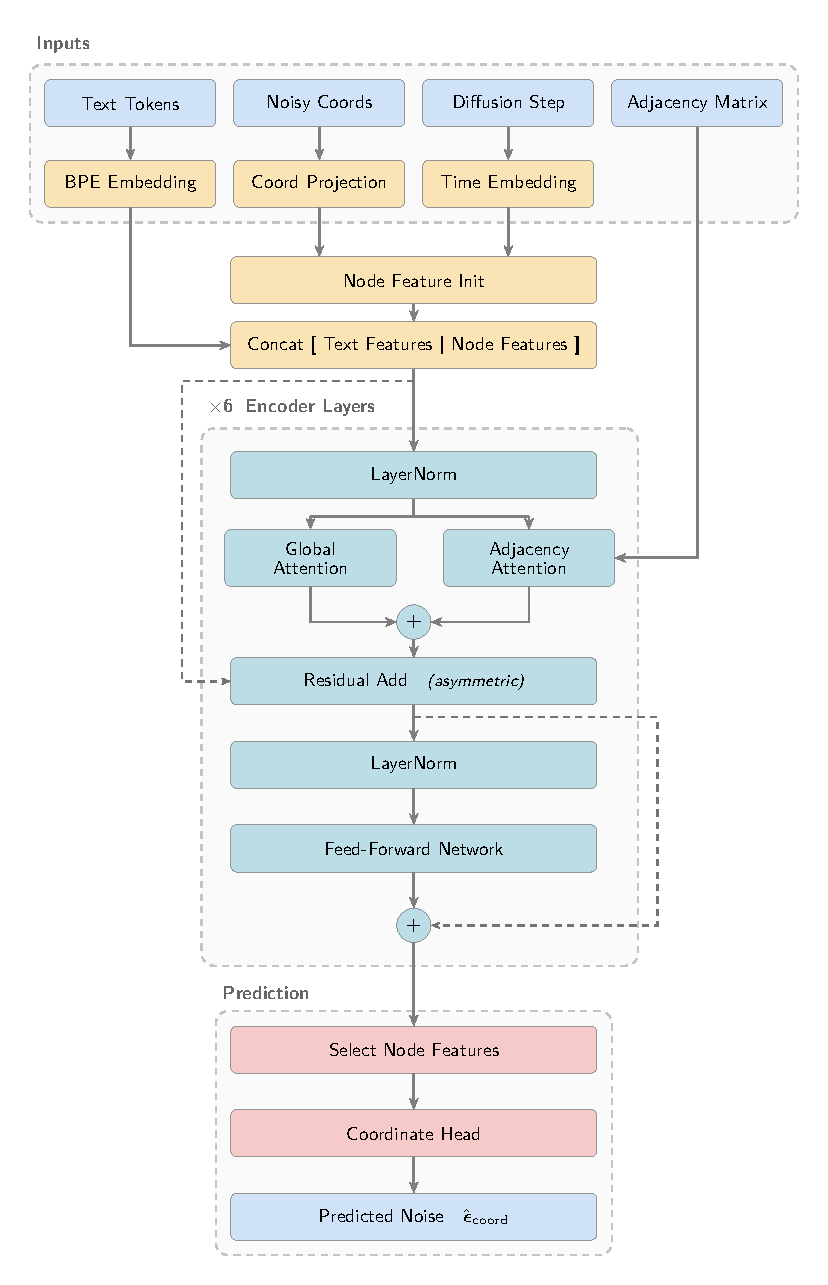
\includegraphics[width=\linewidth]{figures/node_diffusion_arch.pdf}
    \caption{
        NodeDiffusionTransformer 架构图。
        输入的加噪坐标、加噪类型嵌入和时间步在 Fusion 模块融合为节点隐向量，
        拼接文本嵌入后经 6 层双流注意力编码器处理；
        最终节点特征分别经 Coordinate Head 和 Type Embedding Head
        预测两路噪声 $\hat{\boldsymbol{\epsilon}}_{\mathrm{coord}}$ 和
        $\hat{\boldsymbol{\epsilon}}_{\mathrm{type}}$。
    }
    \label{fig:arch}
\end{figure}

\paragraph{节点特征融合}
坐标特征与类型嵌入并非两条独立序列，而是在输入阶段直接相加，
与时间步嵌入共同构成每个节点的\textbf{单一共享隐向量}：
\begin{equation}
    \mathbf{h}_i^{(0)} = W_c\,\mathbf{x}_t^{(i)}
                       + \mathbf{e}_t^{(i)}
                       + \mathrm{MLP}\!\left(\gamma(t)\right)
    \label{eq:node_init}
\end{equation}
其中 $\gamma(t)$ 为正弦时间步编码，$W_c \in \mathbb{R}^{d \times 2}$。
这一设计的关键在于：坐标与类型信息在同一表示空间内相互耦合，
后续所有注意力计算均作用于这一融合向量。
因此，坐标与类型之间并无独立的 cross-attention 流，
而是通过共享向量在每一次注意力计算中隐式耦合。
具体而言，每个注意力头的 Q/K/V 均由融合向量线性投影得到：
\begin{equation}
    \mathbf{Q}_i = W_Q\,\mathbf{h}_i^{(\ell)},\quad
    \mathbf{K}_j = W_K\,\mathbf{h}_j^{(\ell)},\quad
    \mathbf{V}_j = W_V\,\mathbf{h}_j^{(\ell)}
    \label{eq:qkv}
\end{equation}
由于 $\mathbf{h}_j^{(\ell)}$ 同时携带坐标与类型信息，
注意力分数 $\mathbf{Q}_i \cdot \mathbf{K}_j^\top$ 及聚合值
$\sum_j \alpha_{ij}\mathbf{V}_j$ 均隐含了两者的联合感知。
两个输出 head 也均从同一 $\mathbf{h}_i^{(L)}$ 读取，
使坐标噪声预测与类型噪声预测在整个去噪过程中保持相互感知。

\paragraph{双流注意力层}
每层包含两条并行注意力流，输出残差相加后经 FFN 处理：
\begin{equation}
\begin{split}
    \mathbf{h}_i^{(\ell+1)} = \mathbf{h}_i^{(\ell)}
    &+ \mathrm{Dropout}\!\left(\mathrm{AdjAttn}(\mathbf{H}_{\mathrm{node}}^{(\ell)})\right)_{\!i} \\
    &+ \mathrm{Dropout}\!\left(\mathrm{GlobalAttn}(\mathbf{H}_{\mathrm{full}}^{(\ell)})\right)_{\!i}
\end{split}
    \label{eq:dual_attn}
\end{equation}

\begin{itemize}
    \item \textbf{邻接局部注意力 $\mathrm{AdjAttn}$}：
    仅对节点序列 $\mathbf{H}_{\mathrm{node}}$ 计算，
    注意力掩码由邻接矩阵决定：
    \begin{equation}
        M_{ij}^{\mathrm{adj}} =
        \begin{cases}
            0       & \text{若 } \mathbf{A}_{ij} = 1 \\
            -\infty & \text{其他}
        \end{cases}
        \label{eq:adj_mask}
    \end{equation}
    每个节点仅能关注直连邻居，在保证图结构约束的同时，
    使相邻节点之间的坐标与类型特征得以局部交换。

    \item \textbf{全局注意力 $\mathrm{GlobalAttn}$}：
    对拼接序列 $\mathbf{H}_{\mathrm{full}} = [\mathbf{H}_{\mathrm{text}};
    \mathbf{H}_{\mathrm{node}}]$ 做无约束注意力，
    使每个节点能跨越图结构感知全局布局与文本语义，
    并使所有节点的融合特征（含坐标与类型）之间形成完全连接。
    文本嵌入通过可学习 BPE 嵌入层（维度 $d=384$）获得，
    无需预训练语言模型。
\end{itemize}

共堆叠 6 层，model\_channels $= 384$，6 头，dropout $= 0.1$。

\subsubsection{训练目标}

联合训练目标为：
\begin{equation}
    \mathcal{L} = \mathcal{L}_{\mathrm{coord}} + \lambda\,\mathcal{L}_{\mathrm{type}}
    \label{eq:loss}
\end{equation}
\begin{align}
    \mathcal{L}_{\mathrm{coord}}
        &= \frac{\displaystyle\sum_{i} m_i
                 \left\|\hat{\boldsymbol{\epsilon}}_{\mathrm{coord},i}
                       - \boldsymbol{\epsilon}_i\right\|^2}
                {2\displaystyle\sum_i m_i}
    \label{eq:loss_coord} \\[6pt]
    \mathcal{L}_{\mathrm{type}}
        &= \frac{\displaystyle\sum_{i} m_i
                 \left\|\hat{\boldsymbol{\epsilon}}_{\mathrm{type},i}
                       - \boldsymbol{\delta}_i\right\|^2}
                {d\displaystyle\sum_i m_i}
    \label{eq:loss_type}
\end{align}
其中 $m_i$ 为节点有效掩码，$\lambda = 1.0$。
$\mathcal{L}_{\mathrm{type}}$ 在嵌入空间预测类型噪声，
与 $\mathcal{L}_{\mathrm{coord}}$ 共享扩散时间步，
同时起到对坐标预测的语义正则化作用。

优化器为 AdamW（lr $= 10^{-4}$，weight decay $= 10^{-4}$），
grad clip $= 1.0$，batch $= 64$，total steps $= 200\text{k}$，FP16 混合精度。

\subsubsection{推理：坐标采样与类型恢复}

逆过程执行标准 DDPM 采样（1000 步）：
\begin{equation}
    p_{\theta_2}(\mathbf{x}_{t-1} \mid \mathbf{x}_t, \mathbf{A}, \mathcal{T})
    = \mathcal{N}\!\left(\mathbf{x}_{t-1};\,\boldsymbol{\mu}_\theta,\,\tilde{\beta}_t\mathbf{I}\right)
    \label{eq:reverse}
\end{equation}
\begin{equation}
    \boldsymbol{\mu}_\theta = \frac{1}{\sqrt{\alpha_t}}\!\left(
        \mathbf{x}_t - \frac{\beta_t}{\sqrt{1-\bar{\alpha}_t}}
        \hat{\boldsymbol{\epsilon}}_\theta\right)
    \label{eq:mu}
\end{equation}
类型嵌入路同步采样得到 $\hat{\mathbf{e}}_0^{(i)}$，
再通过最近邻查找恢复离散类型：
\begin{equation}
    \hat{y}_i = \arg\min_{k \in \{1,\ldots,32\}}
                \left\|\hat{\mathbf{e}}_0^{(i)} - \mathrm{Emb}(k)\right\|_2
    \label{eq:type_recover}
\end{equation}

% -----------------------------------------------------------------------------
\subsection{推理流程}
\label{subsec:inference}

给定文本 $\mathcal{T}$，完整推理分三步：
（1）Stage~1 自回归生成图序列 token，解析得邻接矩阵 $\mathbf{A}$ 与节点数 $N$；
（2）Stage~2 以 $(\mathbf{A}, \mathbf{m}, \mathcal{T})$ 为条件，
从 $(\mathbf{x}_T, \{\mathbf{e}_T^{(i)}\}) \sim \mathcal{N}(\mathbf{0},\mathbf{I})$
出发执行 1000 步逆扩散，得到节点坐标 $\hat{\mathbf{X}}$ 与类型 $\hat{\mathbf{y}}$；
（3）反归一化坐标，结合 $\mathbf{A}$ 与 $\hat{\mathbf{y}}$ 渲染矢量平面图。

\paragraph{最小度约束}
Stage~1 在生成补边序列（\texttt{SEP} 之后）时，
施加\textbf{最小度约束}：若当前图中存在度数小于 2 的节点，
则在 logit 采样前将 \texttt{EOS\_G} 对应的 logit 置为 $-\infty$，
强制模型继续生成补边，直至所有节点满足 $\deg(v_i) \geq 2$。

该约束的几何动机在于：顶点图中每个节点代表房间多边形的一个角点，
角点至少需连接两条边才能构成有效的多边形转角。
度数为 1 的悬挂节点无法参与闭合多边形的构造，
会导致后处理渲染时出现孤立线段或破碎轮廓。
通过在推理阶段以零额外训练代价强制施加此约束，
可显著提升生成图的几何合法率。

完整推理流程如算法~\ref{alg:inference} 所示。

\begin{algorithm}[t]
\caption{PlanDiffusion 推理}
\label{alg:inference}
\begin{algorithmic}[1]
\REQUIRE 文本描述 $\mathcal{T}$
\ENSURE 节点坐标 $\hat{\mathbf{X}}$，节点类型 $\hat{\mathbf{y}}$，邻接矩阵 $\mathbf{A}$
\STATE \textbf{Stage 1：图拓扑生成}
\STATE 以 $\mathcal{T}$ 为条件，自回归采样生成树序列 token
\WHILE{未采样到 \texttt{EOS\_G}}
    \STATE 采样下一个 token $s \sim p_{\theta_1}(\cdot \mid s_{<k})$
    \IF{$s = \texttt{EOS\_G}$ \AND $\exists\, i: \deg(v_i) < 2$}
        \STATE 将 \texttt{EOS\_G} 的 logit 置为 $-\infty$，重新采样  \COMMENT{最小度约束}
    \ENDIF
\ENDWHILE
\STATE 解析序列得 $\mathbf{A} \in \{0,1\}^{N \times N}$，节点掩码 $\mathbf{m}$
\STATE \textbf{Stage 2：坐标与类型扩散}
\STATE 采样初始噪声 $\mathbf{x}_T \sim \mathcal{N}(\mathbf{0},\mathbf{I})$，$\mathbf{E}_T \sim \mathcal{N}(\mathbf{0},\mathbf{I})$
\FOR{$t = T, T{-}1, \ldots, 1$}
    \STATE $(\hat{\boldsymbol{\epsilon}}_{\mathrm{coord}}, \hat{\boldsymbol{\epsilon}}_{\mathrm{type}}) = f_\theta(\mathbf{x}_t, \mathbf{E}_t, t, \mathbf{A}, \mathbf{m}, \mathcal{T})$
    \STATE $\mathbf{x}_{t-1} \leftarrow$ DDPM 逆步（$\mathbf{x}_t$，$\hat{\boldsymbol{\epsilon}}_{\mathrm{coord}}$，$t$）
    \STATE $\mathbf{E}_{t-1} \leftarrow$ DDPM 逆步（$\mathbf{E}_t$，$\hat{\boldsymbol{\epsilon}}_{\mathrm{type}}$，$t$）
\ENDFOR
\STATE $\hat{\mathbf{X}} \leftarrow \mathbf{x}_0$
\STATE $\hat{y}_i = \arg\min_{k} \|\hat{\mathbf{e}}_0^{(i)} - \mathrm{Emb}(k)\|_2$，$\forall i$
\RETURN $\hat{\mathbf{X}},\; \hat{\mathbf{y}},\; \mathbf{A}$
\end{algorithmic}
\end{algorithm}

\section{实验}
\label{sec:experiments}

\subsection{实验设置}
\label{subsec:setup}

\paragraph{评估指标}
我们从图拓扑合法性、坐标回归精度和节点类型预测三个维度评估各子模块，
并以图结构分布指标衡量端到端生成质量。
所有指标均在 8,000 条独立测试集上计算。

\begin{itemize}
    \item \textbf{图有效率（Graph Validity Rate, GVR）}：
    生成图中连通且无孤立节点的样本占比，反映图拓扑生成的合法性。

    \item \textbf{度分布 KL 散度（Degree KL）}：
    生成图与真实图的节点度分布之间的 KL 散度，
    衡量端到端生成的图结构分布质量。

    \item \textbf{节点数分布 KL 散度（Node-count KL）}：
    生成图与真实图的节点数分布之间的 KL 散度，
    衡量模型对平面图规模的建模能力。

    \item \textbf{坐标 RMSE（Coord-RMSE）}：
    给定真实图结构条件下，去噪预测坐标与真实坐标的均方根误差（像素单位），
    衡量节点坐标扩散子模块的回归精度。

    \item \textbf{类型准确率（Type Acc.）}：
    给定真实坐标和图结构条件下，节点类型预测与真实类型的匹配率，
    衡量类型预测子模块的分类精度。
\end{itemize}

\paragraph{基线方法}
由于本文与现有方法在输入模态上存在根本差异，对比以方法特性说明为主：

\begin{itemize}
    \item \textbf{Architext}~\cite{galanos2023architext}：
    在 Architext\_v1 数据集上微调 GPT 系列模型，以自然语言描述直接生成平面图。
    其文本描述由规则模板生成，语言单一，且不建模显式图结构。

    \item \textbf{HouseDiffusion}~\cite{shabani2023housediffusion}：
    以气泡图（bubble diagram）为条件，通过混合扩散模型生成矢量多边形平面图。
    几何质量优秀，但需手工绘制气泡图，不支持自然语言输入。

    \item \textbf{ChatHouseDiffusion}~\cite{qin2025chathousediffusion}：
    在 HouseDiffusion 基础上引入 prompt 引导，支持文本条件生成与编辑，
    但缺乏对拓扑结构的显式约束。
\end{itemize}

\paragraph{实现细节}
\todo{待补充：训练硬件、训练时长、推理时间。}

\subsection{主实验结果}
\label{subsec:main_results}

\todo{待写：与 Architext 基线的对比。}

\subsection{消融实验}
\label{subsec:ablation}

\todo{待写。}

\subsection{定性结果}
\label{subsec:qualitative}

\todo{待写：生成结果可视化。}

\section{结论}
\label{sec:conclusion}

本文提出了 PlanDiffusion，一种以图结构为中间表示的文本驱动住宅平面图生成框架。
通过将生成任务分解为自回归图拓扑生成（Stage~1）和节点坐标扩散（Stage~2）两个阶段，
本方法在保证房间连通拓扑合法性的同时，实现了从自然语言到矢量平面图的端到端生成。

为支撑模型训练，我们构建了 PlanText-150K 数据集，
包含 149,609 条具有高质量自然语言描述的平面图样本，
是目前规模最大的带文本标注住宅平面图数据集之一。

\todo{实验结果完成后补充定量结论和局限性分析。}

未来工作将探索更长文本条件下的生成质量提升、
多楼层平面图生成，以及基于用户反馈的交互式编辑能力。


% ── 参考文献 ─────────────────────────────────────────────────────────────────
{\small
\bibliographystyle{abbrvnat}
\bibliography{references}
}

\end{document}
